\documentclass[11pt,a4paper]{article}

\usepackage{graphicx}

% ---- Idioma y tipografía
\usepackage[spanish]{babel}
\usepackage[T1]{fontenc}
\usepackage[utf8]{inputenc}  % (si usas XeLaTeX/LuaLaTeX, elimínala)
\usepackage{lmodern}
\usepackage{microtype}

% ---- Márgenes y diseño
\usepackage[a4paper,margin=2.2cm]{geometry}
\usepackage{parskip}

% ---- Enlaces
\usepackage[hidelinks]{hyperref}
\usepackage{bookmark}
% ---- Cabeceras y pies
\usepackage{fancyhdr}
\pagestyle{fancy}
\fancyhf{}
\renewcommand{\headrulewidth}{0.4pt}
\cfoot{\thepage}

% ---- Listas y símbolos
\usepackage{enumitem}
\setlist{itemsep=0.25em, topsep=0.3em}

% ---- Iconos y color
\usepackage{fontawesome5}
\usepackage{xcolor}
\usepackage[most]{tcolorbox}
\tcbuselibrary{breakable,skins}

% ---- Colores propios
\definecolor{uniPrimary}{HTML}{0A7AC3}
\definecolor{uniSoft}{HTML}{E9F4FB}
\definecolor{uniAccent}{HTML}{F5B700}
\definecolor{uniOK}{HTML}{2E7D32}
\definecolor{uniWarn}{HTML}{C62828}

% ---- Metadatos reutilizables
\newcommand{\asignatura}{MULTIMEDIA}
\newcommand{\tema}{TEMA 1 — Conceptos básicos sobre multimedia e Hipermedia}  % <-- cambia el título del tema aquí
\newcommand{\clase}{Clase 1}
\newcommand{\fecha}{\today}                              % <-- pon la fecha de la clase

% ---- Cabecera con metadatos
\lhead{\textsc{\asignatura}}
\rhead{\textbf{\tema}}

% ---- Estética de secciones
\usepackage{titlesec}
\titleformat{\section}{\Large\bfseries\color{uniPrimary}}{\thesection}{0.5em}{}
\titleformat{\subsection}{\large\bfseries}{\thesubsection}{0.5em}{}
\titleformat{\subsubsection}{\bfseries}{\thesubsubsection}{0.5em}{}

% ---- Cajas útiles
\newtcolorbox{ObjetivosBox}{
	title={\faBullseye\; Índice},
	colback=uniSoft,
	colframe=uniPrimary,
	enhanced, breakable,
	left=8pt,right=8pt,top=8pt,bottom=8pt,
	boxrule=0.8pt,
	fonttitle=\bfseries
}

\newtcolorbox{DefBox}{
	title={\faBook\; Definición},
	colback=white,
	colframe=uniAccent,
	enhanced, breakable,
	left=8pt,right=8pt,top=8pt,bottom=8pt,
	boxrule=0.8pt,
	fonttitle=\bfseries
}

\newtcolorbox{NotaBox}{
	title={\faStickyNote\; Nota},
	colback=white,
	colframe=uniPrimary,
	enhanced, breakable,
	left=8pt,right=8pt,top=8pt,bottom=8pt,
	boxrule=0.8pt,
	fonttitle=\bfseries
}

\newtcolorbox{RecordatorioBox}{
	title={\faBell\; Recordatorio},
	colback=uniAccent!15,
	colframe=uniAccent,
	enhanced, breakable,
	left=8pt,right=8pt,top=8pt,bottom=8pt,
	boxrule=0.8pt,
	fonttitle=\bfseries
}

\newtcolorbox{ChecklistBox}{
	title={\faTasks\; Tareas / Checklist},
	colback=white,
	colframe=uniPrimary,
	enhanced, breakable,
	left=8pt,right=8pt,top=8pt,bottom=8pt,
	boxrule=0.8pt,
	fonttitle=\bfseries
}

\newtcolorbox{ResumenBox}{
	title={\faHighlighter\; Resumen rápido (5 líneas)},
	colback=uniSoft,
	colframe=uniPrimary,
	enhanced, breakable,
	left=8pt,right=8pt,top=8pt,bottom=8pt,
	boxrule=0.8pt,
	fonttitle=\bfseries
}

\newtcolorbox{VocabBox}{
	title={\faLanguage\; Vocabulario clave},
	colback=white,
	colframe=uniPrimary,
	enhanced, breakable,
	left=8pt,right=8pt,top=8pt,bottom=8pt,
	boxrule=0.8pt,
	fonttitle=\bfseries
}

% ---- Tabla estilo evaluación (por si la necesitas hoy)
\newcommand{\TablaEvaluacion}{
	\begin{center}
		\renewcommand{\arraystretch}{1.3}
		\begin{tabular}{|l|c|c|c|}
			\hline
			\textbf{Criterio} & \textbf{Porcentaje} & \textbf{Obligatorio} & \textbf{Recuperable} \\
			\hline
			Teoría (25\% cada parcial) & 50\% & Sí & Sí \\
			Práctica & 25\% & Sí & Sí \\
			Aprovechamiento en clase & 10\% & No & No \\
			Trabajo teórico & 15\% & No & Sí \\
			\hline
			\textbf{Total} & \textbf{100\%} &  &  \\
			\hline
		\end{tabular}
	\end{center}
}

% =========================================================
\begin{document}

	% ---- Cabecera de ficha de clase (rellenable en cada sesión)
	{\large \textbf{\asignatura} \;—\; \textbf{\tema} \hfill}\\begin{equation*}0.4em]
	\faUser\; Alumno/a: Alberto Díaz\hfill
	\faChalkboardTeacher\; Profesor/a: Ana Fernández

	\vspace{0.6em}

	\tableofcontents

	% ---- Conceptos clave y definiciones
	\section{Definiciones}
	\begin{DefBox}
		\textbf{Multimedia:} Representación integrada de la información en forma de texto, gráficos, imágenes, vídeo.

		La multimedia no tiene porque ser interactiva. No necesariamente tiene que ser digital.
	\end{DefBox}



	\begin{DefBox}
		\textbf{Aplicación multimedia:} Software capaz de ofrecer información al usuario integrando distintos medios de representación multimedia.

		La información multimedia se procesa y almacena digitalmente.
	\end{DefBox}

	\begin{DefBox}
		\textbf{Elemento Interactivo: } Un elemento es interactivo cuando responde a la entrada de información del usuario. El usuario debe poder tomar una decisión de iniciar la interacción, de forma explicita o implícita.
	\end{DefBox}

	\begin{DefBox}
		\textbf{Hipertexto} Sistema de organización de datos basado en la vinculación de bloques de información llamados nodos.
	\end{DefBox}

	\begin{DefBox}
		\textbf{Hipermedia} Hipertexto + Multimedia. Conectar fragmentos de información que no necesariamente tienen porque ser texto si no cualquier tipo de multimedia.
	\end{DefBox}

	\subsection{Diferencias entre Multimedia, Hipertexto y Hipermedia}

	\begin{center}
		\renewcommand{\arraystretch}{1.4} % más espacio entre filas
		\begin{tabular}{|l|c|c|c|}
			\hline
			\textbf{Criterio} & \textbf{Multimedia} & \textbf{Hipertexto} & \textbf{Hipermedia} \\
			\hline
			\textbf{Contenido}
			& Más de un medio
			& Solo un medio (texto)
			& Más de un medio (texto + otros) \\
			\hline
			\textbf{Enlaces}
			& No
			& Sí (entre textos)
			& Sí (entre distintos medios) \\
			\hline
			\textbf{Navegación}
			& No (Linear)
			& Sí (No linear)
			& Sí \\
			\hline
		\end{tabular}
	\end{center}

	\subsection{Medios multimedia y Contexto}
	\begin{DefBox}
		\textbf{Medio} Canal que permite la distribución y comunicación de la información: Texto, gráficos, imagen, audio y vídeo.
	\end{DefBox}

	\subsubsection{Clasificación en función del tiempo}

	\begin{itemize}[leftmargin=1.5em]
		\item \textbf{Medios continuos (dependientes del tiempo):}
		Requieren una secuencia temporal para ser comprendidos.
		Ejemplos: \textit{audio, vídeo}.

		\item \textbf{Medios discretos (independientes del tiempo):}
		No dependen de la dimensión temporal para interpretarse.
		Ejemplos: \textit{texto, imágenes}.
	\end{itemize}

	\begin{NotaBox}
		\textbf{Contexto:} Esta clasificación se aplica en el ámbito de las \textbf{comunicaciones audiovisuales digitales}.
	\end{NotaBox}

	\subsection*{La importancia del usuario}
	\begin{DefBox}
		\textbf{Percepción} La forma en la que el cerebro interpreta los estímulos del exterior. Las percepciones evocan \textbf{sensaciones}.
	\end{DefBox}

	\begin{DefBox}
		\textbf{Sensaciones} Impresiones que los estímulos externos generan sobre las personas. Percepción de un cambio o desequilibrio.
	\end{DefBox}

	\begin{DefBox}
		\textbf{Emociones} Respuesta que aparece después de la sensación, alegría, tristeza...
	\end{DefBox}

	\textbf{Ejemplo}:
	Veo una nube negra $\rightarrow$ \textit{percepción}.
	Pienso que va a llover $\rightarrow$ \textit{sensación}.
	Me invade la tristeza $\rightarrow$ \textit{emoción}.

	\section{Reseña Histórica}
	Primeras comunicaciones visuales surgían en la prehistoria pero no eran multimedia

	El invento del \textbf{transistor} fue importante para el desarrollo de la multimedia.

	\begin{itemize}[]
		\item \textbf{1945} Vannebar Bush propuso que los computadores deberían usarse como soporte del trabajo intelectual. Almacenamiento y comunicación de contenido multimedia y conocimiento de la humanidad. \textbf{(MEMEX) Memory Extension.}

		\item \textbf{1983} Se desarrolla \textbf{Intermedia}. Programación de creación hipertextual para UNIX.

		\item \textbf{1984} Apple lanza el \textbf{primer Macintosh} con interfaz gráfica. Primera computadora con altas capacidades de reproducción de sonidos y diseño gráfico.

		\item \textbf{1980´s} Aparecen \textbf{videojuegos} y software de entretenimiento.

		\item \textbf{1992} Es posible integrar audio, sonido  y voz, gráficas, animación de texto. Se expande la world wide web.

		\item \textbf{1995-2016} Gran evolución. Aparece el \textbf{metaverso}.
	\end{itemize}

	\subsection{Punto de inflexión: 1995-2000}

	\begin{itemize}[]
		\item Se extiende la señal analógica TV.
		\item \textbf{VHS}: Principal medio para grabar.
		\item Los teléfonos solo tenían llamadas y SMS.
		\item Conexión a internet es lenta. Modem.
		\item Páginas web son \textbf{estáticas}
	\end{itemize}

	\subsection{Punto de inflexión: 2015-2016}

	\begin{itemize}[]
		\item Señal digital de TV
		\item Teléfonos móviles son \textbf{smartphones} con muchas funciones.
		\item Páginas web son sitios interactivos, dinámicas.
		\item Mejor conexión a internet.
		\item Videollamadas.
		\item Se desarrollan las redes sociales.
	\end{itemize}

	\subsection{Punto de inflexión: Escena actual}

	\begin{itemize}[]
		\item Inteligencia Artificial.
		\item Segmentación de imágenes en tiempo real
		\item Realidad Virtual y Aumentada
		\item ChatGPT
	\end{itemize}

\section{Servicios multimedia}

\begin{DefBox}
\textbf{Servicio multimedia:} Permite manejar desde un terminal todas las formas de información electrónica conocidas (texto, gráficos, audio, vídeo, fotografías, música y comunicaciones telefónicas).
Una de sus características principales es la \textbf{interactividad}, que posibilita la comunicación con otras personas o dispositivos.
\end{DefBox}

\subsection{Clasificación de los servicios multimedia}
\begin{itemize}[leftmargin=1.5em]
  \item \textbf{Servicios de broadcasting convencional}
  \item \textbf{Servicios de broadcasting interactivos}
  \item \textbf{Servicios de reproducción multimedia}
  \item \textbf{Servicios de comunicaciones personales}
  \item \textbf{Servicios de juegos}
  \item \textbf{Servicios de monocasting compartido}
\end{itemize}

\subsection{Características principales por tipo}

\subsubsection*{Broadcasting convencional}
\begin{itemize}
  \item Unidireccional
  \item Punto a multipunto
  \item Tiempo real o no
  \item Bajo retraso (no crítico)
  \item Alta calidad
  \item Modelo de producción de contenidos centralizados
  \item Soporte de varios canales y redes
\end{itemize}

\subsubsection*{Broadcasting interactivo}
\begin{itemize}
  \item Bidireccional (asimétrico)
  \item Punto a multipunto y punto a punto
  \item Tiempo real o no
  \item Tiempo de respuesta crítico
  \item Alta calidad
  \item Producción centralizada de contenidos
  \item Uso de múltiples canales y redes
\end{itemize}

\subsubsection*{Reproducción multimedia}
\begin{itemize}
  \item Local (no hay transmisión en red)
  \item Alta capacidad de almacenamiento (p. ej. discos ópticos)
  \item Bajo retraso
  \item Calidad muy alta
\end{itemize}

\subsubsection*{Comunicaciones personales}
Discord, Teams, WhatsApp
\begin{itemize}
  \item Bidireccionales y simétricas
  \item Punto a punto
  \item Tiempo real
  \item Retraso crítico
  \item Calidad media/baja
  \item Contenidos específicos
  \item Soporte de varios canales/redes
\end{itemize}

\subsubsection*{Servicios de juegos}
\begin{itemize}
  \item Bidireccionales (almacenamiento y transmisión)
  \item Punto a punto o multipunto
  \item Tiempo real
  \item Retraso crítico
  \item Alta calidad y realismo
  \item Contenidos sintéticos y reales
  \item Uso de múltiples canales y redes
\end{itemize}

\subsubsection*{Monocasting compartido}
\begin{itemize}
  \item Bidireccional (asimétrico)
  \item Descarga/visionado
  \item Punto a punto
  \item Tiempo real (descarga) y no real (subida)
  \item Retraso crítico
  \item Amplio rango de calidades
  \item Modelo de producción descentralizado y compartido
  \item Uso de múltiples canales/redes sociales
\end{itemize}

El contenido descentralizado se refiere a aquel que es generado y distribuido por múltiples usuarios o entidades independientes, en lugar de depender de una única fuente central. Por ejemplo, plataformas como Netflix gestionan y controlan todo su catálogo (contenido centralizado), mientras que en YouTube cualquier usuario puede crear y compartir vídeos, lo que constituye un modelo de contenido descentralizado.

\section{Señales analógicas vs digitales}

\begin{DefBox}
\textbf{Señales analógicas:} Representan fenómenos continuos de la naturaleza (voz, luz, temperatura, etc.). Son percibidas directamente por el ser humano a través de los sentidos.
Se caracterizan por ser infinitas en valores y difíciles de controlar totalmente.
\end{DefBox}

\begin{DefBox}
\textbf{Señales digitales:} Representación discreta de una señal analógica mediante procesos de \textbf{muestreo}, \textbf{cuantificación} y \textbf{codificación}.
Permiten mayor control, almacenamiento y transmisión eficiente.
\end{DefBox}

\subsection{Características principales}

\subsubsection*{Señales analógicas}
\begin{itemize}
  \item Continuas en el tiempo y en amplitud.
  \item Utilizadas en sistemas tradicionales de comunicación (TV, radio, teléfono).
  \item Menor control sobre la calidad (ruido, distorsión, interferencias).
  \item Requieren equipos especializados para almacenamiento y transmisión.
\end{itemize}

\subsubsection*{Señales digitales}
\begin{itemize}
  \item Discretas en el tiempo y en amplitud (valores finitos representados en bits).
  \item Flexibles gracias al procesado por software.
  \item Almacenamiento sencillo y de gran capacidad.
  \item Permiten compresión y transmisión eficiente.
  \item Menor degradación en transmisión y copias.
\end{itemize}

\subsection{Ventajas de lo digital frente a lo analógico}
\begin{ChecklistBox}
\begin{itemize}
  \item Mayor \textbf{flexibilidad}: procesamiento mediante software frente al hardware analógico.
  \item Implementación de algoritmos avanzados de procesado de señal.
  \item Reducción de costes a largo plazo.
  \item Facilidad de almacenamiento masivo.
  \item Menor sensibilidad al ruido e interferencias.
\end{itemize}
\end{ChecklistBox}

\subsection{Proceso de conversión}
\begin{itemize}
  \item \textbf{Muestreo:} Se toma la señal analógica a intervalos regulares de tiempo.
  \item \textbf{Cuantificación:} Se aproxima el valor muestreado a un nivel discreto predeterminado.
  \item \textbf{Codificación:} Representación en bits de cada valor cuantificado.
\end{itemize}

\begin{NotaBox}
Si el emisor y el receptor son humanos, se requiere \textbf{ADC (Conversor Analógico-Digital)} en la entrada y \textbf{DAC (Conversor Digital-Analógico)} en la salida.
Si ambos son dispositivos electrónicos, la transmisión puede permanecer en el dominio digital.
\end{NotaBox}

\begin{ResumenBox}
Las señales analógicas son naturales y continuas, pero difíciles de controlar.
Las digitales permiten un manejo más eficiente y robusto, gracias a la conversión mediante muestreo, cuantificación y codificación.
Su ventaja radica en la flexibilidad, el almacenamiento y la resistencia al ruido.
\end{ResumenBox}

\subsection{Teorema de Nyquist}

\begin{DefBox}
\textbf{Teorema de Nyquist:}
Para poder reconstruir una señal analógica a partir de sus muestras digitales, la \textbf{frecuencia de muestreo} $F_m$ debe ser al menos el doble del \textbf{ancho de banda} $B$ de la señal original:

\[
F_m > 2B
\end{equation*}

Esto garantiza una representación digital adecuada y evita pérdidas de información.
\end{DefBox}

\subsubsection*{Conceptos clave}
\begin{itemize}
  \item \textbf{Ancho de banda ($B$):} Rango de frecuencias presentes en la señal.
  \item \textbf{Frecuencia de muestreo ($F_m$):} Número de muestras tomadas por segundo.
  \item \textbf{Aliasing:} Distorsión que ocurre si se muestrea a una frecuencia inferior a $2B$.
  Algunas frecuencias de la señal original se confunden con otras diferentes al reconstruir la señal.
\end{itemize}

\subsubsection*{Ejemplo práctico}
\begin{itemize}
  \item La voz humana tiene un ancho de banda aproximado de $3\,\text{kHz}$.
  \item Según Nyquist: $F_m > 2 \times 3\,\text{kHz} = 6\,\text{kHz}$.
  \item En telefonía digital se usa una frecuencia de muestreo estándar de $8\,\text{kHz}$ para asegurar una buena calidad.
\end{itemize}

\begin{NotaBox}
Cuanto mayor es la frecuencia de muestreo, más fiel será la representación de la señal, pero también mayor será el \textbf{bit rate} y el almacenamiento necesario.
Por ello, se busca un compromiso entre calidad y eficiencia.
\end{NotaBox}

\begin{ResumenBox}
El teorema de Nyquist establece que debemos muestrear al doble de la frecuencia máxima de la señal para evitar aliasing.
Es la base de toda digitalización de audio, vídeo y otros datos multimedia.
\end{ResumenBox}

\subsection{Cuantificación}

\begin{DefBox}
\textbf{Cuantificación:}
Proceso mediante el cual, tras el muestreo de una señal analógica, cada valor continuo se aproxima al \textbf{nivel discreto más cercano}.
De esta forma, los valores de la señal se representan con un número finito de niveles llamados \textbf{niveles de cuantificación}.
\end{DefBox}

\subsubsection*{Conceptos clave}
\begin{itemize}
  \item La cuantificación convierte una secuencia de muestras continuas en un conjunto finito de valores discretos.
  \item El número de niveles de cuantificación $N$ depende del número de bits $b$ utilizados:
  \begin{equation*}
  N = 2^b
  \end{equation*}
  \item Cada muestra tiene un \textbf{error de cuantificación}:
  \begin{equation*}
  e(T) = x_{\text{analógica}}(T) - x_{\text{cuantificada}}(T)
  \end{equation*}
  Cuantos más bits se usan, menor es el error, pero mayor el espacio necesario para almacenamiento o transmisión.
\end{itemize}

\subsubsection*{Tipos de cuantificación}
\begin{itemize}
  \item \textbf{Uniforme:} Los niveles están equiespaciados.
  Se utiliza en imágenes o datos en general.
  \item \textbf{No uniforme:} Los niveles no están equiespaciados; se adaptan a la señal.
  Muy útil en audio, ya que hay muchas amplitudes cercanas a cero (silencios).
  \item \textbf{Midtread:} Tiene un nivel de cuantificación en cero.
  Adecuado para señales con muchas muestras alrededor del valor cero (como audio).
  \item \textbf{Midrise:} No tiene nivel en cero, el número de niveles es par.
\end{itemize}

\subsubsection*{Ejemplo}
\begin{itemize}
  \item Para un cuantificador de 2 bits ($b=2$):
  \begin{equation*}
  N = 2^2 = 4 \text{ niveles discretos}
  \end{equation*}
  La señal se aproxima solo a 4 valores posibles, lo que genera un error de cuantificación alto.
  \item Si se usan 8 bits, se obtienen $2^8 = 256$ niveles, con una representación mucho más fiel.
\end{itemize}

\begin{NotaBox}
La \textbf{calidad de la cuantificación} se mide con la relación señal-ruido (SNR).
Se cumple que, aproximadamente, la SNR mejora \textbf{6 dB por cada bit adicional} en el cuantificador.
\end{NotaBox}

\begin{ResumenBox}
La cuantificación aproxima cada muestra a un nivel discreto predeterminado.
A mayor número de bits, menor error y mayor calidad, pero también mayor consumo de memoria y ancho de banda.
\end{ResumenBox}

% ------------------------------------------------------------
% Sección ampliada: cuantificación, bitrate y SNR
% ------------------------------------------------------------
\subsection{Cuantificación: bitrate y SNR}

La \emph{cuantificación} asigna cada muestra analógica a uno de los $2^N$ niveles
posibles, donde $N$ es el número de bits por muestra. En audio PCM (modulación por
impulso codificado), el \textbf{bitrate} (tasa de bits) viene dado por:
\begin{equation}
  R \;=\; f_s \cdot N \cdot C \quad [\text{bits/s}]
\end{equation}
donde $f_s$ es la frecuencia de muestreo (muestras por segundo),
$N$ los bits por muestra, y $C$ el número de canales (por ejemplo, $C=2$ en estéreo).
Para pasar a bytes por segundo, dividir entre 8.

\paragraph{Ejemplos de bitrate PCM sin compresión}
\begin{itemize}
  \item \textbf{CD audio estéreo}: $f_s=44{,}1$ kHz, $N=16$, $C=2$ \\
    $R = 44{,}100 \times 16 \times 2 = 1{,}411{,}200\ \text{bits/s} \approx 1{,}411\ \text{kbit/s}$ \\
    $= 176{,}400\ \text{B/s} \approx 172{,}27\ \text{KiB/s} \approx 10{,}09\ \text{MiB/min}$.
  \item \textbf{44{,}1 kHz, 16 bits, mono} ($C=1$):\\
    $R = 44{,}100 \times 16 \times 1 = 705{,}600\ \text{bits/s} \approx 706\ \text{kbit/s}$ \\
    $\approx 5{,}05\ \text{MiB/min}$.
  \item \textbf{Estándar de producción} $48$ kHz, $24$ bits, estéreo ($C=2$):\\
    $R = 48{,}000 \times 24 \times 2 = 2{,}304{,}000\ \text{bits/s} \approx 2{,}304\ \text{kbit/s}$ \\
    $= 288{,}000\ \text{B/s} \approx 16{,}48\ \text{MiB/min}$.
  \item \textbf{Alta resolución} $96$ kHz, $24$ bits, estéreo: \\
    $R = 96{,}000 \times 24 \times 2 = 4{,}608{,}000\ \text{bits/s} \approx 4{,}608\ \text{kbit/s}$ \\
    $= 576{,}000\ \text{B/s} \approx 32{,}96\ \text{MiB/min}$.
\end{itemize}

\paragraph{Bitrates típicos en audio con compresión (referencia)}
Estos valores no siguen la fórmula anterior porque usan codificación perceptual (con o sin pérdidas):
\begin{itemize}
  \item \textbf{MP3}: 128, 192, 256, 320 kbit/s (estéreo).
  \item \textbf{AAC}: 128--256 kbit/s (estéreo) para buena calidad; en streaming es común 256 kbit/s.
  \item \textbf{Opus}: 64--160 kbit/s (estéreo) según calidad/latencia; voz mono a menudo 16--32 kbit/s.
\end{itemize}

\paragraph{Cuantización y ruido: SNR teórico}
La cuantificación uniforme introduce un error de redondeo que se modela como ruido blanco acotado.
Para una \textbf{señal senoidal a escala completa} (full-scale), el \textbf{SNR de cuantificación} ideal es:
\begin{equation}
  \mathrm{SNR}_q \;\approx\; 6{,}02\,N + 1{,}76 \quad [\text{dB}].
\end{equation}
De esta relación se desprende que cada bit adicional aporta $\approx 6$ dB de mejora en SNR.

\paragraph{Ejemplos de SNR teórico}
\begin{itemize}
  \item $N=8$ bits $\Rightarrow \mathrm{SNR}_q \approx 6{,}02\times 8 + 1{,}76 \approx 49{,}9\ \text{dB}$.
  \item $N=16$ bits $\Rightarrow \mathrm{SNR}_q \approx 98{,}1\ \text{dB}$ (típico de CD en el mejor caso).
  \item $N=24$ bits $\Rightarrow \mathrm{SNR}_q \approx 146{,}2\ \text{dB}$ (límite teórico; en la práctica
        el ruido analógico del convertidor/previos reduce esta cifra).
\end{itemize}

\paragraph{ENOB (número efectivo de bits)}
En sistemas reales, el SNR medido puede traducirse a \emph{bits efectivos}:
\begin{equation}
  \mathrm{ENOB} \;=\; \frac{\mathrm{SNR}_{\text{medido}} - 1{,}76}{6{,}02}.
\end{equation}
\emph{Ejemplo}: si se mide $\mathrm{SNR}=90$ dB, entonces $\mathrm{ENOB}\approx (90-1{,}76)/6{,}02 \approx 14{,}7$ bits.

\paragraph{Notas prácticas}
\begin{itemize}
  \item Subir $f_s$ aumenta el \emph{bitrate} linealmente; subir $N$ mejora el \emph{SNR} teórico $\approx 6$ dB/bit.
  \item \emph{Dither} y \emph{noise shaping} pueden mejorar artefactos perceptuales al reducir a menor $N$.
  \item En compresión con pérdidas (p.\,ej., MP3/AAC/Opus) el \emph{bitrate} ya no depende de $f_s$, $N$ y $C$ de forma directa:
        el códec descarta información psicoacústicamente redundante para alcanzar el objetivo en kbit/s.
\end{itemize}

% (Opcional) Tabla rápida de bitrates PCM comunes.
\begin{table}[h!]
\centering
\begin{tabular}{lccc}
\hline
\textbf{Formato} & $f_s$ (kHz) & $N$ (bits) & \textbf{Bitrate} (kbit/s) \\
\hline
Mono ``CD-like''     & 44{,}1 & 16 & 706 \\
Estéreo CD           & 44{,}1 & 16 & 1{,}411 \\
Estéreo producción   & 48     & 24 & 2{,}304 \\
Estéreo alta resolución & 96  & 24 & 4{,}608 \\
\hline
\end{tabular}
\caption{Bitrates PCM sin compresión típicos (aprox.).}
\end{table}

\section{Redundancias en la señal}

\begin{DefBox}
\textbf{Redundancia espacial:} Dentro de una imagen una sección puede contener píxeles iguales o similares, por lo que, si codificamos cada píxel de igual manera, estaríamos enviando información redundada.
\end{DefBox}

\begin{DefBox}
\textbf{Redundancia temporal:} En el vídeo, fotogramas consecutivos pueden presentar gran similitud; hay información repetida a lo largo de los fotogramas.
\end{DefBox}

\begin{DefBox}
\textbf{Redundancia:} Presencia de información repetida o predecible en los datos que puede ser eliminada (sin o con mínima pérdida perceptual) para reducir la tasa binaria sin afectar significativamente la calidad percibida.
\end{DefBox}

\begin{NotaBox}
Nota, parte de la información de la señal es irrelevante desde el punto de vista perceptivo. Por ejemplo, ciertos cambios de tonalidades entre ciertos colores son casi imperceptibles al ojo humano. En las imagenes borrosas los detalles son imperceptibles por lo que no es necesario enviar una gran cantidad de información para generar la misma percepción
\end{NotaBox}

\subsection{Sistemas de Compresión}

\begin{DefBox}
Sistema de compresión CODE, consta de codificador y decodificador, EnCOder y DECoder.
\end{DefBox}

\textbf{Tipos:}
\begin{itemize}
	\item Asimétricos, el codificador tarda mucho en codificar y poco en descodificar.
	\item Simétricos, Coste computacional similar.
	\item Con pérdidas o irreversible; mayores tasas de compresión, Video e Imagenes, JPEG, MPEG.
	\item Sin pérdidas o reversible. Tasas de compresión moderadas. Texto, ZIP
\end{itemize}

\subsection{Sistemas genéricos de compresión}
\begin{itemize}
	\item \textbf{Análisis:} Representación eficaz que facilita la compresión.
	\item \textbf{Cuantificador:} Conversión a valores discretos.
	\item \textbf{Asignación de palabras de código:} Series de bits utilizados para representar los niveles de cuantificación.
\end{itemize}

Este es el proceso de codificación. La decodificación es el mismo proceso pero a la inversa.

\section{Tipos de datos multimedia}

\begin{NotaBox}
Habitualmente se asocia con los datos de audio video e image, pero también se puede considerar texto o gráficos.

Los datos multimedia pueden ser \textbf{continuos} o \textbf{estáticos}.

Las aplicaciones multimedia basadas en datos continuos representan mayores retos y requerimientos, retardos, sincronismo, etc...
\end{NotaBox}

\subsection {Gráficos}
\begin{DefBox}
\textbf{Gráficos vectoriales:} Representación basada en \textbf{primitivas geométricas} (puntos, líneas, curvas, polígonos) definidas mediante coordenadas y fórmulas matemáticas. \\
\textbf{Características principales:}
\begin{itemize}[leftmargin=1.3em]
	\item Independientes de la resolución (reescalado sin pérdida de calidad).
	\item Ficheros ligeros para formas simples.
	\item Ideales para: logotipos, tipografía, iconos, diagramas, ilustración técnica.
	\item Formatos habituales: SVG, PDF, EPS, AI.
\end{itemize}
\end{DefBox}

\begin{DefBox}
\textbf{Gráficos raster (mapa de bits):} Representación mediante una rejilla (matriz) de píxeles, cada uno con un valor de color. \\
\textbf{Características principales:}
\begin{itemize}[leftmargin=1.3em]
	\item Dependientes de la resolución (al ampliar se percibe pixelación / pérdida aparente de calidad).
	\item Adecuados para: fotografías, texturas, arte complejo con variaciones tonales.
	\item Tamaño del fichero crece con la resolución y profundidad de color.
	\item Formatos habituales: PNG, JPEG, BMP, GIF, TIFF.
\end{itemize}
\end{DefBox}

\begin{ResumenBox}
Vector: objetos geométricos, escalable, ideal para diseño limpio. \\
Raster: píxeles, depende de la resolución, ideal para fotografía. \\
La elección depende de: tipo de contenido, necesidad de escalado y optimización.
\end{ResumenBox}

% (Opcional) Comparativa rápida
\begin{center}
\renewcommand{\arraystretch}{1.25}
\begin{tabular}{|l|c|c|}
\hline
\textbf{Aspecto} & \textbf{Vector} & \textbf{Raster} \\
\hline
Escalado & Perfecto & Pierde nitidez \\
Detalle fotográfico & Limitado & Excelente \\
Edición de formas & Muy precisa & Limitada \\
Tamaño (formas simples) & Muy reducido & Mayor \\
Uso típico & Logo / Iconos & Fotografía \\
\hline
\end{tabular}
\end{center}

\subsection{Texto}

\begin{DefBox}
\textbf{Texto digital:} Secuencia de \emph{puntos de código} (code points) pertenecientes a un \textbf{repertorio} (conjunto abstracto de caracteres) que se materializa mediante una \textbf{codificación} (mapping a bytes). El mismo carácter puede representarse con distinto número de bytes según el estándar.
\end{DefBox}

\subsubsection*{Evolución de codificaciones}
\begin{itemize}[leftmargin=1.4em]
	\item \textbf{ASCII (7 bits, 1963)}: 128 símbolos (0–127). Letras inglesas, dígitos, control.
	\item \textbf{ASCII extendido (8 bits)}: 256 posiciones (0–255). No estandarizado globalmente: distintas páginas de códigos (Latin-1, CP1252, ISO-8859-x, etc.).
	\item \textbf{Unicode (ISO/IEC 10646)}: Repertorio universal (más de 149k caracteres). Asigna un \emph{code point} U+XXXX.
	\item \textbf{UTF-8}: Codificación de Unicode de longitud variable (1–4 bytes). Retrocompatible con ASCII (0x00–0x7F).
	\item \textbf{UTF-16}: 16 bits.
	\item \textbf{UTF-32}: 32 bits.
\end{itemize}

También se pueden codificar las palabras con otros sistemas como EBCDIC (IBM) o GB18030 (chino).

\subsection{Audio}

\begin{DefBox}
\textbf{Audio:} Onda acústica (variación de presión en un medio, típicamente aire) que se modela como señal \textbf{unidimensional} en el tiempo. Un \textbf{transductor} (micrófono) convierte estas variaciones en señal eléctrica que luego se digitaliza (muestreo, cuantificación y codificación). El oído humano percibe frecuencias aproximadamente entre \textbf{20 Hz} y \textbf{20 kHz}.
\end{DefBox}

\begin{NotaBox}
La señal puede captarse en \textbf{mono} (un canal) o en \textbf{estéreo} (dos canales sincronizados).
\end{NotaBox}

\subsubsection*{Ejemplo: Telefonía digital (PCM)}
\begin{DefBox}
La voz telefónica se limita (filtra) aproximadamente al rango 200--3200 Hz para reducir ancho de banda y evitar componentes innecesarias. Según Nyquist, la frecuencia de muestreo debe ser mayor al doble de la frecuencia máxima: $F_s > 2 \times 3200 = 6400$ Hz. Se estandariza $F_s = 8000$ Hz.
\end{DefBox}

\begin{NotaBox}
Bitrate (tasa binaria) PCM sin compresión (mono):
\begin{equation*}
R = F_s \times N = 8000\ \text{muestras/s} \times 8\ \text{bits/muestra} = 64{,}000\ \text{bits/s} = 64\ \text{kbit/s}
\end{equation*}
Este es el caudal básico de la telefonía digital tradicional (PCM G.711 antes de compresión adicional).
\end{NotaBox}

\begin{ChecklistBox}
\begin{itemize}
	\item Banda voz (filtrada): 200--3200 Hz
	\item Frecuencia Nyquist mínima: > 6400 Hz
	\item Frecuencia usada: 8000 Hz
	\item Profundidad de cuantificación: 8 bits
	\item Bitrate resultante: 64 kbit/s (PCM lineal teórico)
\end{itemize}
\end{ChecklistBox}

\begin{ResumenBox}
Filtrar la voz reduce el ancho de banda requerido. Muestrear a 8 kHz y cuantificar a 8 bits produce 64 kbit/s, base de la telefonía digital clásica.
\end{ResumenBox}

\subsection{Imagenes}

Con imágenes nos referimos a \textit{mapas de bits rasterizados} representados mediante matrices de píxeles.
Cada píxel puede tener un distinto número de canales, por ejemplo:
\begin{itemize}
    \item \textbf{Monocromáticas:} 1 canal (imágenes en blanco y negro).
    \item \textbf{Imágenes a color:} 3 canales (RGB o HSV).
\end{itemize}

Las imágenes pueden estar en gran cantidad de formatos que utilizan distintos modelos de color, tales como:
\begin{equation*}
\text{RGB, HSV, CMYK, YUV}
\end{equation*}

\subsection{Video}

Se trata de una \textbf{secuencia de imágenes}, donde las frecuencias más comunes son:

\begin{equation*}
24 \ \text{fps}, \quad 30 \ \text{fps}, \quad 60 \ \text{fps}
\end{equation*}

Esta frecuencia garantiza la \textit{percepción visual} y proporciona una sensación de \textbf{continuidad}.

\section{Audio}
La magnitud en decibelios (dB) se define como:

\begin{equation*}
\text{dB} = 20 \cdot \log_{10}\!\left(\frac{A}{B}\right)
\end{equation*}

donde $A$ es la amplitud medida y $B$ es la amplitud de referencia.

\begin{itemize}
    \item $0 \,\text{dB}$: umbral mínimo de audición.
    \item $120 \,\text{dB}$: umbral del dolor.
\end{itemize}

\subsection*{Voz vs Música}

\textbf{Voz}
\begin{itemize}
    \item Servicios de tecnología telefónica.
    \item Estándar \textbf{G.711}.
    \item Codificación logarítmica (\textit{µ-law} y \textit{A-law}).
    \item Parámetros:
    \begin{itemize}
        \item Ancho de banda: $3.5 \,\text{KHz}$.
        \item Tasa de bits: $64 \,\text{Kbps}$.
    \end{itemize}
\end{itemize}

\textbf{Música}
\begin{itemize}
    \item Calidad de audio superior.
    \item Codificación lineal.
\end{itemize}

\section{Video}

\subsection{Vídeo análogo}

Es una sucesión de imágenes que producen la sensación de movimiento. La imagen está compuesta de ondas electromagnéticas; diferentes longitudes de onda producen diferentes sensaciones de color.

\begin{itemize}
	\item Las imágenes son convertidas en una señal analógica en intervalos de tiempo regulares.
	\item Para reproducir la imagen se realiza el proceso inverso.
	\item Parámetros de barrido:
		\begin{itemize}
			\item Relación de aspecto: 4:3, 16:9 (ancho:alto).
			\item Algunas líneas, superiores e inferiores, no se ven.
			\item Estándares: NTSC (525 líneas), PAL (625 líneas).
			\item Frecuencia de refresco: 50 Hz (PAL), 60 Hz (NTSC).
		\end{itemize}
	\item Parpadeo de imagen (\textit{flicker}):
		\begin{itemize}
			\item Se produce por la baja frecuencia de refresco.
			\item Se soluciona con el barrido entrelazado: primero líneas pares y luego impares.
		\end{itemize}
\end{itemize}

\subsection{Vídeo digital}

\begin{itemize}
	\item Parámetros de barrido:
	\begin{itemize}
		\item Dos formatos: NTSC y PAL.
		\item Resolución: 720$\times$480 (NTSC), 525$\times$825 (PAL).
		\item Frecuencia de refresco: 50 Hz (PAL), 60 Hz (NTSC).
	\end{itemize}
\end{itemize}

\subsection{Formatos de color}

El formato \textbf{RGB} parte de la idea de que cualquier color puede ser representado por una combinación de los colores primarios: rojo, verde y azul.
En la representación digital, cada color primario se cuantifica en un número determinado de bits, normalmente 8 bits, es decir, 24 bits por píxel.

El formato \textbf{YUV} se compone de:
\begin{itemize}
    \item $Y$: Luminancia
    \item $U$: Componente azul
    \item $V$: Componente rojo
\end{itemize}

La conversión entre RGB y YUV se expresa mediante la siguiente matriz de transformación:

\begin{equation}
\begin{bmatrix}
Y \\[6pt]
U \\[6pt]
V
\end{bmatrix}
=
\begin{bmatrix}
0.299 & 0.587   & 0.114 \\
-0.14713 & -0.28886 & 0.436 \\
0.615 & -0.51499 & -0.10001
\end{bmatrix}
\cdot
\begin{bmatrix}
R \\[6pt]
G \\[6pt]
B
\end{bmatrix}
\end{equation}

\begin{figure}[h!]
    \centering
    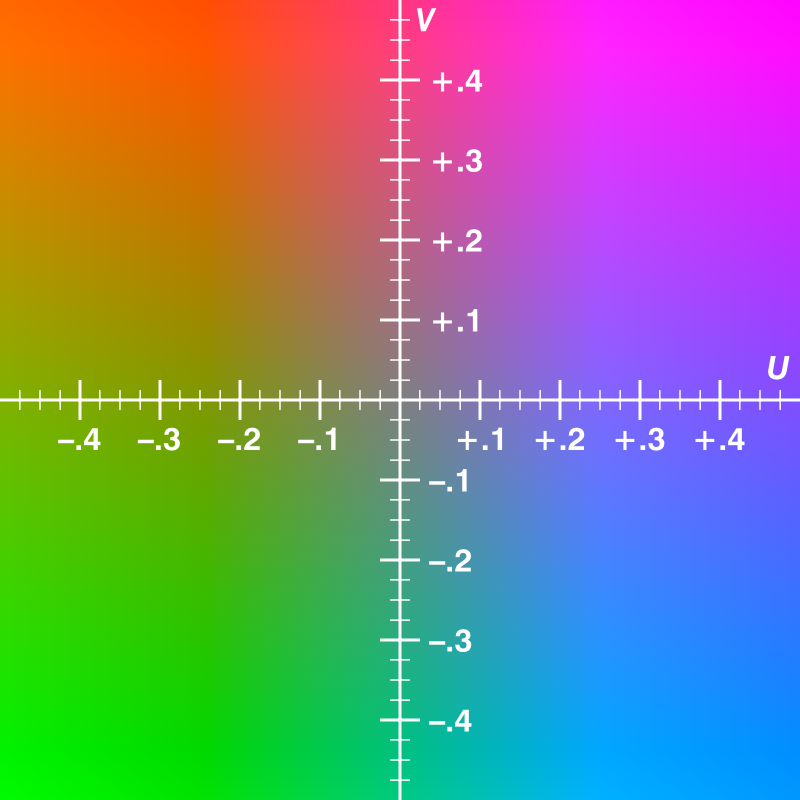
\includegraphics[width=0.5\textwidth]{resources/YUV_UV_plane.png}
    \caption{Plano UV del modelo de color YUV}
    \label{fig:yuv_uv_plane}
\end{figure}

\subsection{Video entrelazado (i) y progresivo (p)}

\textbf{Entrelazado}
\begin{itemize}
    \item Se escanean las líneas impares y luego las pares.
    \item Es más eficiente en movimientos rápidos entre \textit{frames}.
    \item Las líneas espacialmente adyacentes no lo son temporalmente.
\end{itemize}

\textbf{Progresivo}
\begin{itemize}
    \item No existe el concepto de \textit{frame}, se envía todo de forma progresiva.
    \item Se necesita más caudal de datos para la misma calidad.
    \item Se ve mejor el movimiento, pero puede aparecer \textit{tearing}.
\end{itemize}

\section{Técnicas y métricas de calidad visual}

Existen tres tipos:
\begin{itemize}
    \item \textbf{Full reference}: se tiene la imagen original y se compara con la distorsionada.
    \item \textbf{No reference}: no se dispone de la imagen original, solo de la distorsionada.
    \item \textbf{Reduced reference}: se conocen algunas propiedades de la señal original.
\end{itemize}

Las métricas \textbf{full reference} más comunes son:
\begin{itemize}
    \item Error cuadrático medio (MSE, \textit{Mean Square Error}).
    \item Relación señal a ruido (SNR, \textit{Signal to Noise Ratio}).
    \item Relación señal a ruido pico (PSNR, \textit{Peak Signal to Noise Ratio}).
\end{itemize}

\subsection{Métricas subjetivas}

Estas métricas no se ajustan a la calidad subjetiva observada por el ojo humano.

La métrica subjetiva más utilizada es el \textbf{MOS} (\textit{Mean Opinion Score}).

\subsection{Métricas objetivas}

\begin{itemize}
    \item \textbf{Ratio de compresión (en porcentaje):}
    \[
        \text{RC\%} = \frac{\text{Tamaño comprimido}}{\text{Tamaño original}} \times 100 \%
    \]

    \item \textbf{Factor de compresión:}
    \[
        \text{FC} = \frac{\text{Tamaño original}}{\text{Tamaño comprimido}}
    \]

	Expresado como FC:1 (por ejemplo, 10:1).

    \item \textbf{Bits por píxel (bpp):}
    \[
        \text{bpp} = \frac{\text{Número de bits de la imagen codificada}}{\text{Número de píxeles en la imagen original}}
    \]
\end{itemize}

\subsection{Estándares internacionales}

Organizaciones importantes:
\begin{itemize}
    \item ISO (\textit{International Organization for Standardization})
    \item IEC (\textit{International Electrotechnical Commission})
    \item ITU (\textit{International Telecommunication Union})
\end{itemize}

\end{document}
